\documentclass{article}

\usepackage[utf8]{inputenc}
\usepackage{wrapfig}
\usepackage{lscape}
\usepackage{graphicx}
\usepackage{caption}
\usepackage{amsmath, amssymb, amsfonts}
\usepackage{mathtools}
\usepackage{comment}
\usepackage{afterpage}
\usepackage{multirow}
\usepackage{multicol}
% cleveref moved after hyperref
\usepackage{makecell}
\usepackage{booktabs}
\usepackage{longtable}
\usepackage{placeins}
\usepackage{adjustbox}
\usepackage{ragged2e}
\usepackage{enumitem}
\usepackage[a4paper, top=2.54cm, bottom=2.54cm, left=2.54cm, right=2.54cm]{geometry}
\usepackage{hyperref}
\usepackage{cleveref}

\hypersetup{
    colorlinks=true,
    linkcolor=black,
    citecolor=blue,
    urlcolor=blue
}

\newcommand\myemptypage{
    \null
    \thispagestyle{empty}
    \addtocounter{page}{-1}
    \newpage
}

\thispagestyle{empty}
\pagenumbering{arabic}

\begin{document}

\renewcommand{\thepage}{\roman{page}}

% =========================================================================
% TITLE PAGE
% =========================================================================
\begin{titlepage}
\begin{center}
    \centering     
    \vspace*{0.5cm}
    {\LARGE \textbf{BONE FRACTURE IMAGE CAPTIONING USING\\ DEEP LEARNING}\par}
    \vspace{1.0cm}
     
    {\Large \textbf{A PROJECT REPORT}\par}
    \vspace{0.4cm}
    {\large \textit{Submitted in partial fulfilment of the requirements for the award of the degree of}\par}
    \vspace{0.2cm}
    {\Large \textbf{BACHELOR OF TECHNOLOGY}\par}
    {\large \textbf{in}\par}
    {\Large \textbf{COMPUTER SCIENCE AND ENGINEERING}\par}
    \vspace{0.8cm}
   
    {\large \textbf{Submitted by}\par}
    \vspace{0.2cm}
    {\large \textbf{RAJESWARI MOHAPATRA \quad (Regd. No. 240301120019)}\par} 
    {\large \textbf{DONIPUDI ASISH KUMAR \quad (Regd. No. 240301120025)}\par}
    {\large \textbf{YAMANA TANMAY \quad (Regd. No. 240301120059)}\par}
    \vspace{0.8cm}
    
    {\large \textit{Under the guidance of}\par}
    \vspace{0.2cm}
    {\Large \textbf{Dr. Chinmayee Dora}\par}
    {\normalsize Head of the Department, SoC.DS\par}
    \vspace{0.8cm}

    \IfFileExists{images/cutm_logo.png}{
        
\includegraphics[width=0.26\linewidth]{images/cutm_logo.png}
    }{
        \fbox{\parbox{4cm}{\centering \vspace{0.5cm}\textbf{CENTURION UNIVERSITY LOGO}\vspace{0.5cm}}}
    }
    \vspace{0.6cm}

    {\large \textbf{SCHOOL OF ENGINEERING AND TECHNOLOGY}\par}
    {\large \textbf{BHUBANESWAR CAMPUS}\par}
    {\large \textbf{CENTURION UNIVERSITY OF TECHNOLOGY AND MANAGEMENT}\par}
    {\large \textbf{ODISHA, INDIA}\par}
    \vspace{0.4cm}
    {\large \textbf{APRIL 2026}}
\end{center}
\end{titlepage}

\newpage

% =========================================================================
% BONAFIDE CERTIFICATE
% =========================================================================
\section*{}
\addcontentsline{toc}{section}{Bonafide Certificate}
\begin{center}
{\huge \textbf{DEPARTMENT OF COMPUTER SCIENCE AND ENGINEERING}}\par\vspace{0.4cm}
\normalsize
\textsc{SCHOOL OF ENGINEERING AND TECHNOLOGY\\
BHUBANESWAR CAMPUS}\par\vspace{1.5cm}

\underline{\LARGE \textbf{BONAFIDE CERTIFICATE}}\par\vspace{1.2cm}
\end{center}

\normalsize Certified that this project report \textbf{``Bone Fracture Image Captioning Using Deep Learning''} is the bonafide work of \textbf{RAJESWARI MOHAPATRA (240301120019)}, \textbf{DONIPUDI ASISH KUMAR (240301120025)}, and \textbf{YAMANA TANMAY (240301120059)} who carried out the project work under my supervision. This is to further certify to the best of my knowledge, that this project has not been carried out earlier in this institute and the university.\par\vspace{1.5cm}

\begin{flushright}
\textbf{SIGNATURE}\par\vspace{1.2cm}
\textbf{(Dr. Chinmayee Dora)}\\
Head Of The Department, SoC.DS\\
School of Engineering and Technology\par\vspace{1.5cm}
\end{flushright}

\textit{Certified that the above mentioned project has been duly carried out as per the norms of the college and statutes of the university.}\par\vspace{1.5cm}

\begin{flushright}
\textbf{SIGNATURE}\par\vspace{1.2cm}
\textbf{(Dr. Rahul Ray)}\\
Dean of the School / Head of the Department\\
Professor of Computer Science and Engineering
\end{flushright}

\vfill
\newpage

% =========================================================================
% DECLARATION
% =========================================================================
\section*{}
\addcontentsline{toc}{section}{Declaration}
\begin{center}
\underline{\LARGE \textbf{DECLARATION}}\par\vspace{1.5cm}
\end{center}

\large{We hereby declare that the project entitled \textbf{``Bone Fracture Image Captioning Using Deep Learning''}, submitted as part of the Bachelor of Technology programme in Computer Science and Engineering, is our academic project work. The report acknowledges the sources used and presents experimental results according to the project records available. It does not claim that the system has been clinically validated or that it replaces professional radiological assessment. This work has not formed the basis for the award of any other Degree, Diploma, or fellowship in any other University or Institution.}\par\vspace{1.0cm}

\begin{table}[h]
\centering
\begin{tabular}{clc}
\toprule
\textbf{Sl. No.} & \textbf{Name of the Student} & \textbf{Registration Number} \\
\midrule
1. & Rajeswari Mohapatra & 240301120019 \\
2. & Donipudi Asish Kumar & 240301120025 \\
3. & Yamana Tanmay & 240301120059 \\
\bottomrule
\end{tabular}
\end{table}

\vspace{1.5cm}
\noindent \textbf{Place:} Bhubaneswar\par\vspace{0.3cm}
\noindent \textbf{Date:} 

\vfill
\newpage

% =========================================================================
% ACKNOWLEDGEMENTS
% =========================================================================
\section*{}
\addcontentsline{toc}{section}{Acknowledgements}
\begin{center}
\underline{\LARGE \textbf{ACKNOWLEDGEMENTS}}\par\vspace{1.5cm}
\end{center}

\large{We express our sincere gratitude to \textbf{Dr. Chinmayee Dora} for her insightful guidance, constant encouragement, and constructive feedback throughout the course of this project. We thank \textbf{Dr. Rahul Ray}, Dean and Professor, along with the faculty members of the Department of Computer Science and Engineering, and the School of Engineering and Technology, Bhubaneswar Campus, for their academic support and facilitating computational resources.\par

We also acknowledge the researchers and dataset maintainers whose open benchmark contributions supported this project---specifically the Mendeley Data team for the \textit{BoneFract} dataset and the authors of the \textit{FracAtlas} benchmark---along with the open-source software communities maintaining PyTorch, TorchVision, FastAPI, and Streamlit.\par

Finally, we express our heartfelt thanks to our families and friends for their constant encouragement, patience, and understanding during our academic journey.}\par\vspace{1.0cm}

\begin{table}[h]
\centering
\begin{tabular}{clc}
\toprule
\textbf{Sl. No.} & \textbf{Name of the Student} & \textbf{Registration Number} \\
\midrule
1. & Rajeswari Mohapatra & 240301120019 \\
2. & Donipudi Asish Kumar & 240301120025 \\
3. & Yamana Tanmay & 240301120059 \\
\bottomrule
\end{tabular}
\end{table}

\vspace{1.5cm}
\noindent \textbf{Place:} Bhubaneswar\par\vspace{0.3cm}
\noindent \textbf{Date:}

\newpage

% =========================================================================
% ABSTRACT
% =========================================================================
\section*{}
\addcontentsline{toc}{section}{Abstract}
\begin{center}
\underline{\LARGE \textbf{ABSTRACT}}\par\vspace{1.0cm}
\end{center}

Bone fractures are commonly assessed using radiographs, but automated analysis is affected by anatomical variation, image quality, resolution, and class distribution. This project, \textit{Bone Fracture Image Captioning Using Deep Learning}, implements an experimental computer-vision application that predicts binary fracture status and anatomical region, provides a separate candidate-localisation component, and generates a concise caption from supported model outputs.

The principal classifier uses a multi-task architecture with a shared feature extractor and separate outputs for fracture classification and seven anatomical regions: Arm, Foot, Hand, Lower leg, Thigh, Pelvis, and Wrist. The documented experiments include a baseline ResNet-50 at 224$\times$224, Experiment 3 ResNet-50 at 448$\times$448, Experiment 4 balanced ResNet-50 at 448$\times$448, and Experiment 5 Inception-v3 at 299$\times$299. A separate Faster R-CNN detector with a MobileNetV3-FPN backbone is documented for localisation using FracAtlas data. Caption generation is deterministic and rule-based; it is not a trained CNN--LSTM or Transformer language model.

The BoneFract dataset contains 47,931 images in the documented split: 38,366 training, 4,787 validation, and 4,778 held-out test images. A resolution audit records 34,542 images (72.07\%) at native 102$\times$102 resolution. On the documented test partition, Experiment 4 achieved 72.87\% recall, 64.39\% precision, 80.49\% accuracy, 68.36\% F1-score, ROC-AUC 0.8733, PR-AUC 0.7980, and 80.83\% anatomical accuracy. Experiment 3 achieved higher accuracy (81.88\%) and ROC-AUC (0.8770), illustrating the trade-off between sensitivity and false positives. The software test record reports 69 passing automated tests and eight warnings; these tests do not establish clinical validity. The application is an academic prototype and is not intended to replace qualified medical assessment.\par\vspace{0.8cm}
\noindent \textbf{Keywords:} bone fracture, radiographs, ResNet-50, Inception-v3, multi-task learning, object detection, deterministic caption generation, FastAPI, Streamlit.

\newpage

% =========================================================================
% LISTS & TABLES OF CONTENTS
% =========================================================================
\tableofcontents
\newpage
\listoffigures
\newpage
\listoftables
\newpage

\renewcommand{\thepage}{\arabic{page}}
\setcounter{page}{1}

% =========================================================================
% 1. INTRODUCTION
% =========================================================================
\section{Introduction}

\subsection{Problem Statement}
The project addresses the development of an experimental system that accepts a bone X-ray image, predicts one of seven anatomical regions and binary fracture status, optionally returns candidate regions from a separate detector, and displays the results in a web application. The system must distinguish image-level classification from bounding-box localisation and must not generate unsupported clinical details.

\subsection{Objectives of the Project}
The objectives are to:
\begin{enumerate}[noitemsep]
    \item Prepare and document the classification and localisation datasets.
    \item Implement consistent image preprocessing for the selected model input sizes.
    \item Train and compare the documented ResNet-50 and Inception-v3 experiments.
    \item Evaluate fracture classification and anatomical-region prediction on the held-out test partition.
    \item Integrate the separate Faster R-CNN localisation component.
    \item Generate deterministic captions based only on available model outputs.
    \item Integrate inference using FastAPI and a Streamlit interface.
\end{enumerate}

\subsection{Scope of the Project}
The classifier predicts binary fracture status and one of seven dataset-defined anatomical regions. The detector is a separate component for candidate-region localisation. Caption generation uses deterministic rules. The system does not independently infer fracture subtype, laterality, displacement, or severity, and external clinical validation has not been documented.

\subsection{Proposed Solution}
The application follows an image-input, validation, preprocessing, model-inference, caption-generation, and result-display pipeline. The documented resolution-aware gate uses a 300-pixel minimum-dimension threshold: the high-resolution path uses a 448-pixel input and the low-resolution path uses a 224-pixel input. The active production configuration documented in the project guide selects Experiment 3 for the high-resolution branch; Experiment 4 is the recall-leading experimental model but should not be described as deployed unless the registry is changed and verified.

% =========================================================================
% 2. LITERATURE SURVEY
% =========================================================================
\section{Literature Survey}

\subsection{Deep Learning in Bone Fracture Analysis}
Deep-learning methods use learned image representations to classify radiographs and identify visual patterns associated with fractures. In this project, the primary task is binary fracture classification alongside anatomical-region prediction. The supplied literature matrix primarily covers general image captioning; it should therefore be used to explain caption-generation approaches, not as direct evidence that a particular captioning method is clinically validated for fracture radiographs.

\subsection{Existing Fracture Classification Approaches}
Fracture classification systems commonly formulate the task as image-level classification, while localisation systems predict candidate regions. These outputs answer different questions: classification estimates whether a fracture is present in an image, whereas localisation identifies an image region associated with a detector prediction. The project implements these as separate components and evaluates classification using a held-out test partition.

\subsection{CNN-Based Medical Image Analysis}
Convolutional neural networks learn hierarchical visual features through convolutional and pooling operations. ResNet-50 \cite{he2016deep} uses residual connections to support deeper feature extraction, while Inception-v3 \cite{szegedy2016rethinking} uses parallel convolutional paths at multiple scales. The project evaluates these architectures through the documented experiments rather than assuming one architecture is inherently superior.

\subsection{Object Detection and Fracture Localisation}
Faster R-CNN \cite{ren2015faster} combines region proposals with classification and bounding-box regression. The project uses a Faster R-CNN implementation with a MobileNetV3-FPN backbone \cite{howard2019searching, lin2017feature} for the separate localisation task and FracAtlas \cite{rahman2023fracatlas} annotations. Detector metrics must be taken from the detector's own evaluation report; classification metrics cannot be substituted for detection performance.

\subsection{Medical Image Captioning}
The supplied literature matrix describes CNN--LSTM encoder--decoder systems, semantic attention, reference-based captioning, multi-task captioning, and other attention-based approaches. Foundational examples listed in the matrix include \textit{Show and Tell: A Neural Image Caption Generator} (2015) \cite{vinyals2015show} and \textit{Image Captioning With Semantic Attention} (2016) \cite{you2016image}. Such methods generally combine visual features with a language decoder or semantic guidance.

The present project differs from learned captioning systems because its caption generator is deterministic and rule-based. It selects bounded text templates from classifier and, where available, detector outputs. It does not use a trained LSTM, Transformer, or external language model.

\subsection{Research Gap}
The supplied literature matrix mainly describes general image-captioning methods and datasets, rather than direct, controlled comparisons on the BoneFract fracture task. The engineering gap addressed here is the constrained integration of classification and localisation outputs into a readable caption while avoiding unsupported claims. A further project-specific issue is the large low-resolution image subgroup and its lower reported recall. No claim is made that the project outperforms the reviewed publications.

\begin{table}[htbp]
\centering
\caption{Summary of Reviewed Literature on Image Captioning and Medical Vision}
\label{tab:lit_survey}
\resizebox{\textwidth}{!}{
\begin{tabular}{llll}
\toprule
\textbf{Year} & \textbf{Paper Title} & \textbf{Method} & \textbf{Relevance as Summarised in the Matrix} \\
\midrule
2015 & Show and Tell: A Neural Image Caption Generator \cite{vinyals2015show} & CNN encoder, LSTM decoder & Encoder--decoder foundation for image captioning. \\
2016 & Image Captioning With Semantic Attention \cite{you2016image} & CNN features \& semantic attention & Adds semantic attention to visual information. \\
2017 & Reference Based LSTM for Image Captioning \cite{chen2017reference} & CNN and reference-based LSTM & Uses reference/context information. \\
2017 & Semantic Compositional Networks for Visual Captioning \cite{gan2017semantic} & Semantic concepts and LSTM & Conditions text generation on semantic concepts. \\
2018 & A Multi-task Learning Approach for Image Captioning \cite{wang2018multitask} & Multi-task visual \& language learning & Shares learning objectives across caption-related tasks. \\
2018 & Fine-Grained \& Semantic-Guided Visual Attention \cite{wu2018finegrained} & Guided visual attention \& LSTM & Combines fine-grained visual and semantic features. \\
2020 & Efficient CNN-LSTM using Network Compression \cite{liu2020efficient} & Compressed CNN--LSTM & Investigates efficient model execution. \\
2021 & Parallel-fusion LSTM for Image Captioning \cite{zhao2021parallel} & Parallel-fusion LSTM & Fuses semantic and visual information. \\
2022 & Image Caption Generator using CNN and LSTM \cite{sharma2022image} & CNN--LSTM & Applies an encoder--decoder captioning pipeline. \\
2025 & When Better Eyes Lead to Blindness \cite{bhatt2025better} & CNN--LSTM with attention & Examines limits of backbone upgrades for caption quality. \\
\bottomrule
\end{tabular}
}
\end{table}

% =========================================================================
% 3. PROPOSED METHODOLOGY
% =========================================================================
\section{Proposed Methodology}

\subsection{Overall System Workflow}
The system starts with radiographic image input and applies image validation and preprocessing. The multi-task classifier predicts anatomical region and binary fracture status. The separate detector returns candidate bounding boxes when its output meets the implemented criteria. A deterministic caption engine converts supported outputs into text, and the FastAPI backend returns the result to the Streamlit BoneSight interface.

\begin{figure}[htbp]
\centering
\IfFileExists{images/fig_system_architecture.png}{
    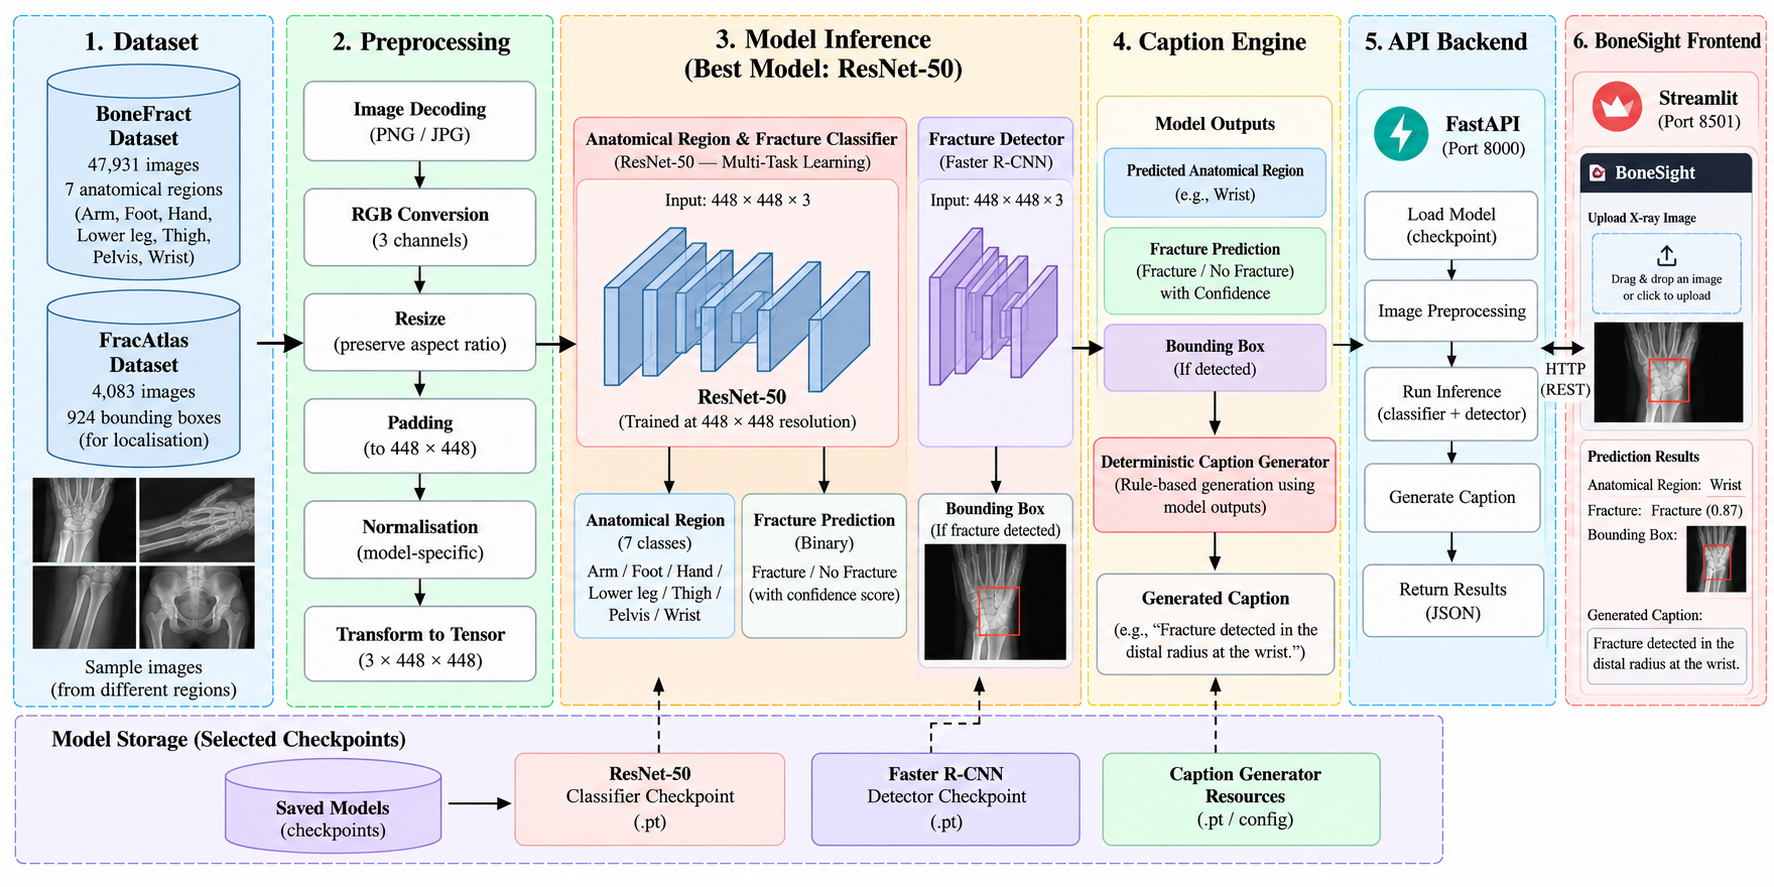
\includegraphics[width=0.95\linewidth]{images/fig_system_architecture.png}
}{
    \fbox{\parbox{0.9\linewidth}{\centering \vspace{0.4cm}\textbf{Figure 3.1: System Architecture Diagram}\par \small (Dataset $\to$ Preprocessing $\to$ Inference $\to$ Caption Engine $\to$ FastAPI $\to$ Streamlit)\vspace{0.4cm}}}
}
\caption{System architecture showing dataset, classifier, detector, API, caption engine, and BoneSight frontend.}
\label{fig:arch}
\end{figure}

\subsection{Dataset Acquisition and Description}
The documented BoneFract classification dataset \cite{bonefract2023} contains 47,931 images across seven anatomical regions. Its recorded partition contains 38,366 training images, 4,787 validation images, and 4,778 held-out test images. The project resolution audit records 34,542 images (72.07\%) at native 102$\times$102 resolution.

\begin{table}[htbp]
\centering
\caption{Documented BoneFract Classification Partition}
\label{tab:bonefract_partition}
\begin{tabular}{lr}
\toprule
\textbf{Partition} & \textbf{Images} \\
\midrule
Training & 38,366 \\
Validation & 4,787 \\
Held-out test & 4,778 \\
\midrule
\textbf{Total} & \textbf{47,931} \\
\bottomrule
\end{tabular}
\end{table}

FracAtlas \cite{rahman2023fracatlas} is documented as the source for the separate detector, with 4,083 images and 924 bounding boxes in the project inventory. The classification and localisation datasets are treated separately because they use different supervision and evaluation procedures.

\subsection{Data Inspection and Label Taxonomy}
The classifier uses seven region labels: Arm, Foot, Hand, Lower leg, Thigh, Pelvis, and Wrist. The data pipeline checks image readability, dimensions, labels, duplicates, and split membership. The project guide records a split audit reporting no patient overlap and no MD5 collisions; these statements should be retained with their audit artefacts for verification.

\subsection{Data Preprocessing}
The documented pipeline decodes images, converts grayscale images to three-channel inputs, resizes while preserving aspect ratio, pads to the required canvas, and applies model-specific normalisation. Experiment input sizes are 224$\times$224 for the baseline ResNet-50, 448$\times$448 for Experiments 3 and 4, and 299$\times$299 for Experiment 5. The detector path is documented at 384$\times$384. Resizing and padding avoid non-uniform stretching, but interpolation cannot recover detail missing from a low-resolution source.

\begin{figure}[htbp]
\centering
\IfFileExists{images/fig_preprocessing_pipeline.png}{
    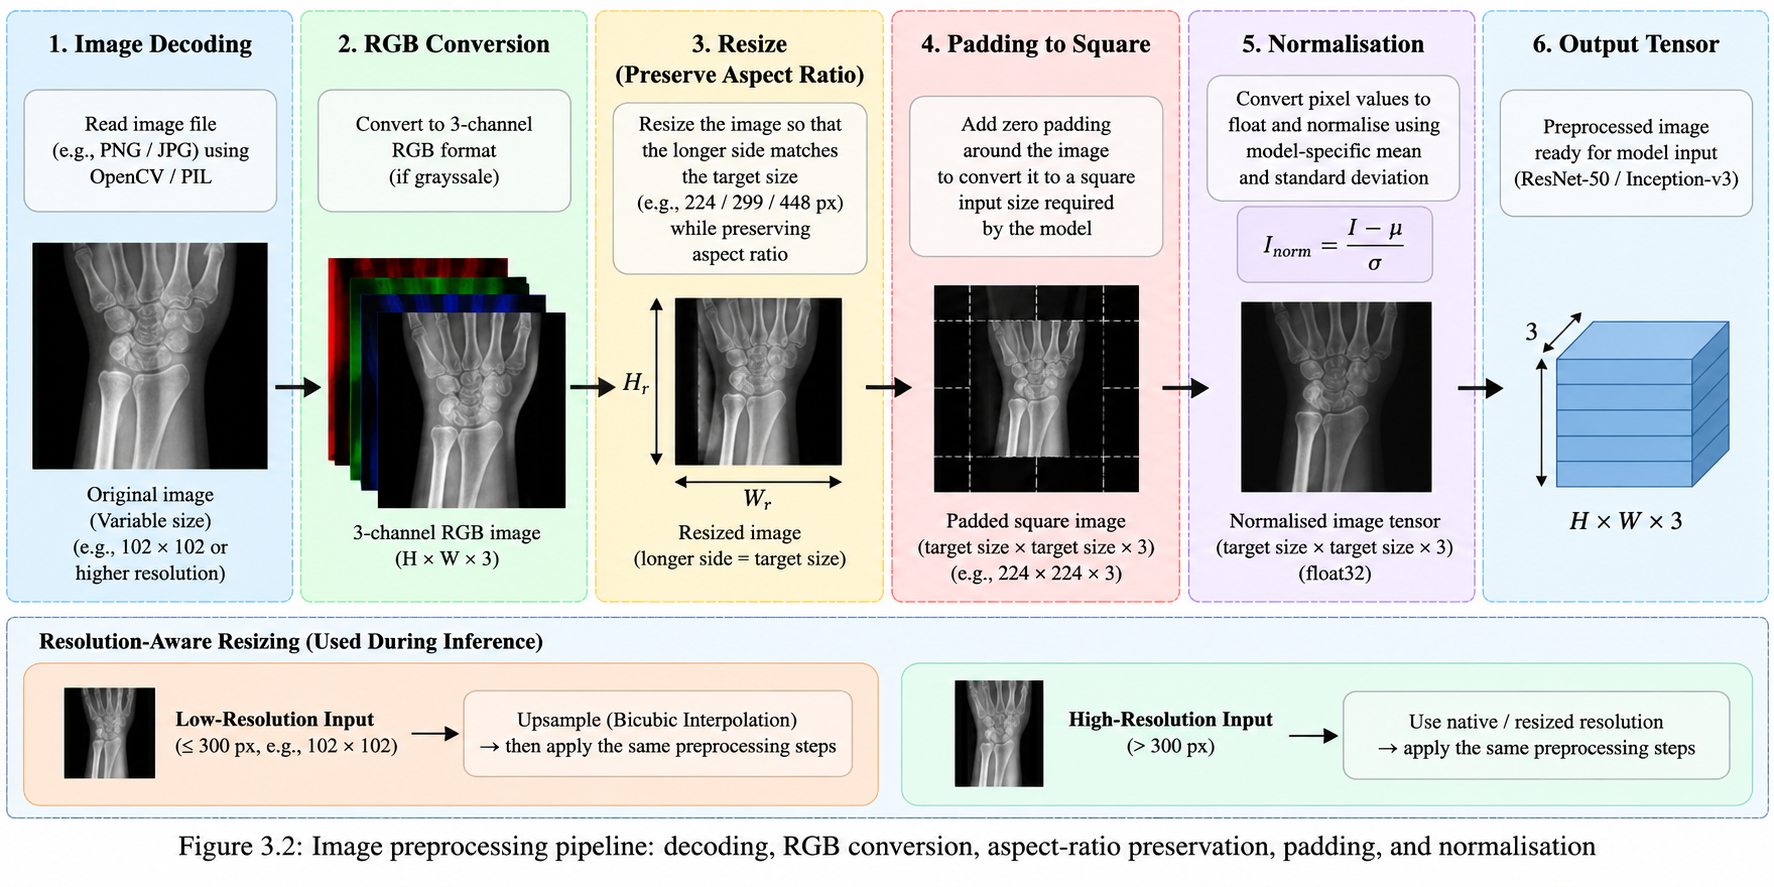
\includegraphics[width=0.95\linewidth]{images/fig_preprocessing_pipeline.png}
}{
    \fbox{\parbox{0.9\linewidth}{\centering \vspace{0.4cm}\textbf{Figure 3.2: Image Preprocessing Pipeline}\par \small (Decoding $\to$ RGB Conversion $\to$ Aspect-Ratio Preserving Resize $\to$ Padding $\to$ Normalisation)\vspace{0.4cm}}}
}
\caption{Image preprocessing pipeline: decoding, RGB conversion, aspect-ratio preservation, padding, and normalisation.}
\label{fig:preprocessing}
\end{figure}

\subsection{Multi-Task ResNet-50 Architecture}
ResNet-50 \cite{he2016deep} is used as a shared feature extractor with task-specific outputs for seven-class anatomical classification and binary fracture prediction. The region head produces a distribution over the anatomical classes, while the fracture head produces a binary score. The shared representation allows both tasks to learn from the image, but correct region prediction does not guarantee correct fracture classification.

The documented Experiment 3 objective combines the anatomical classification loss and a weighted binary fracture loss:
\begin{equation}
\mathcal{L}_{\text{total}} = \mathcal{L}_{\text{region}} + 1.5 \, \mathcal{L}_{\text{fracture}}
\end{equation}
The configuration records a positive-class weight of 2.438 for the binary task. The exact training configuration and code remain the authoritative implementation record.

\subsection{Inception-v3 Architecture}
Experiment 5 uses a multi-task Inception-v3 model \cite{szegedy2016rethinking} with a 299$\times$299 input. It provides an alternative convolutional feature extractor and is compared against the ResNet-50 experiments on the documented held-out partition. The comparison is empirical; architecture choice alone does not imply superior performance.

\subsection{Faster R-CNN for Fracture Localisation}
The localisation component uses Faster R-CNN \cite{ren2015faster} with a MobileNetV3-Large backbone \cite{howard2019searching} and Feature Pyramid Network \cite{lin2017feature}. It is trained separately on FracAtlas bounding-box annotations \cite{rahman2023fracatlas}. The project guide documents a detector confidence threshold of 0.10, which is distinct from the classifier's binary threshold of 0.50. The available evidence summarised for this report does not provide a complete detector metric set, so no detector mAP or localisation accuracy is asserted.

\subsection{Training Experiments and Configurations}
The documented experiments are:
\begin{itemize}[noitemsep]
    \item \textbf{Baseline:} ResNet-50, 224$\times$224 input, full classification training set.
    \item \textbf{Experiment 3:} ResNet-50, 448$\times$448 input, checkpoint \texttt{exp3\_resnet50\_448.pt}.
    \item \textbf{Experiment 4:} region-balanced ResNet-50, 448$\times$448 input, 14,000 images with 2,000 per region.
    \item \textbf{Experiment 5:} multi-task Inception-v3, 299$\times$299 input.
\end{itemize}

Experiment 4 records 6,657 fracture-positive and 7,343 fracture-negative images in its 14,000-image training subset. Training used three head warm-up epochs with a frozen backbone, followed by fine-tuning of layer 4. The run lasted 21 epochs; its highest validation PR-AUC was 0.8168 at epoch 9, and adaptive early stopping triggered at epoch 21.

\begin{table}[htbp]
\centering
\caption{Experiment 4 Region-Balanced Training Distribution}
\label{tab:exp4_distribution}
\begin{tabular}{lrrr}
\toprule
\textbf{Region} & \textbf{Positive} & \textbf{Negative} & \textbf{Total} \\
\midrule
Arm & 785 & 1,215 & 2,000 \\
Foot & 1,000 & 1,000 & 2,000 \\
Hand & 875 & 1,125 & 2,000 \\
Lower leg & 1,000 & 1,000 & 2,000 \\
Thigh & 1,000 & 1,000 & 2,000 \\
Pelvis & 997 & 1,003 & 2,000 \\
Wrist & 1,000 & 1,000 & 2,000 \\
\midrule
\textbf{Total} & \textbf{6,657} & \textbf{7,343} & \textbf{14,000} \\
\bottomrule
\end{tabular}
\end{table}

\subsection{Evaluation Metrics}
The reported binary metrics include recall, specificity, accuracy, precision, F1-score, ROC-AUC, and PR-AUC. With $\text{TP}$, $\text{TN}$, $\text{FP}$, and $\text{FN}$ denoting true positives, true negatives, false positives, and false negatives:
\begin{align}
\text{Precision} &= \frac{\text{TP}}{\text{TP} + \text{FP}} \\
\text{Recall} &= \frac{\text{TP}}{\text{TP} + \text{FN}} \\
\text{Specificity} &= \frac{\text{TN}}{\text{TN} + \text{FP}} \\
\text{Accuracy} &= \frac{\text{TP} + \text{TN}}{\text{TP} + \text{TN} + \text{FP} + \text{FN}} \\
\text{F}_1 &= 2 \cdot \frac{\text{Precision} \cdot \text{Recall}}{\text{Precision} + \text{Recall}}
\end{align}
Anatomical classification accuracy is reported separately from fracture classification metrics. All metrics describe the documented dataset evaluation and do not establish clinical validity.

\subsection{Resolution-Aware Inference}
The documented routing threshold is 300 pixels based on the minimum image dimension. Images meeting the high-resolution condition use the 448-pixel branch; smaller images use the 224-pixel branch. The active production configuration recorded in the project guide uses Experiment 3 for the high-resolution path and \texttt{best\_model.pt} for the low-resolution path. Experiment 4 has the highest reported recall but is not identified as the active production checkpoint in that configuration.

\begin{figure}[htbp]
\centering
\IfFileExists{images/fig_resolution_routing.png}{
    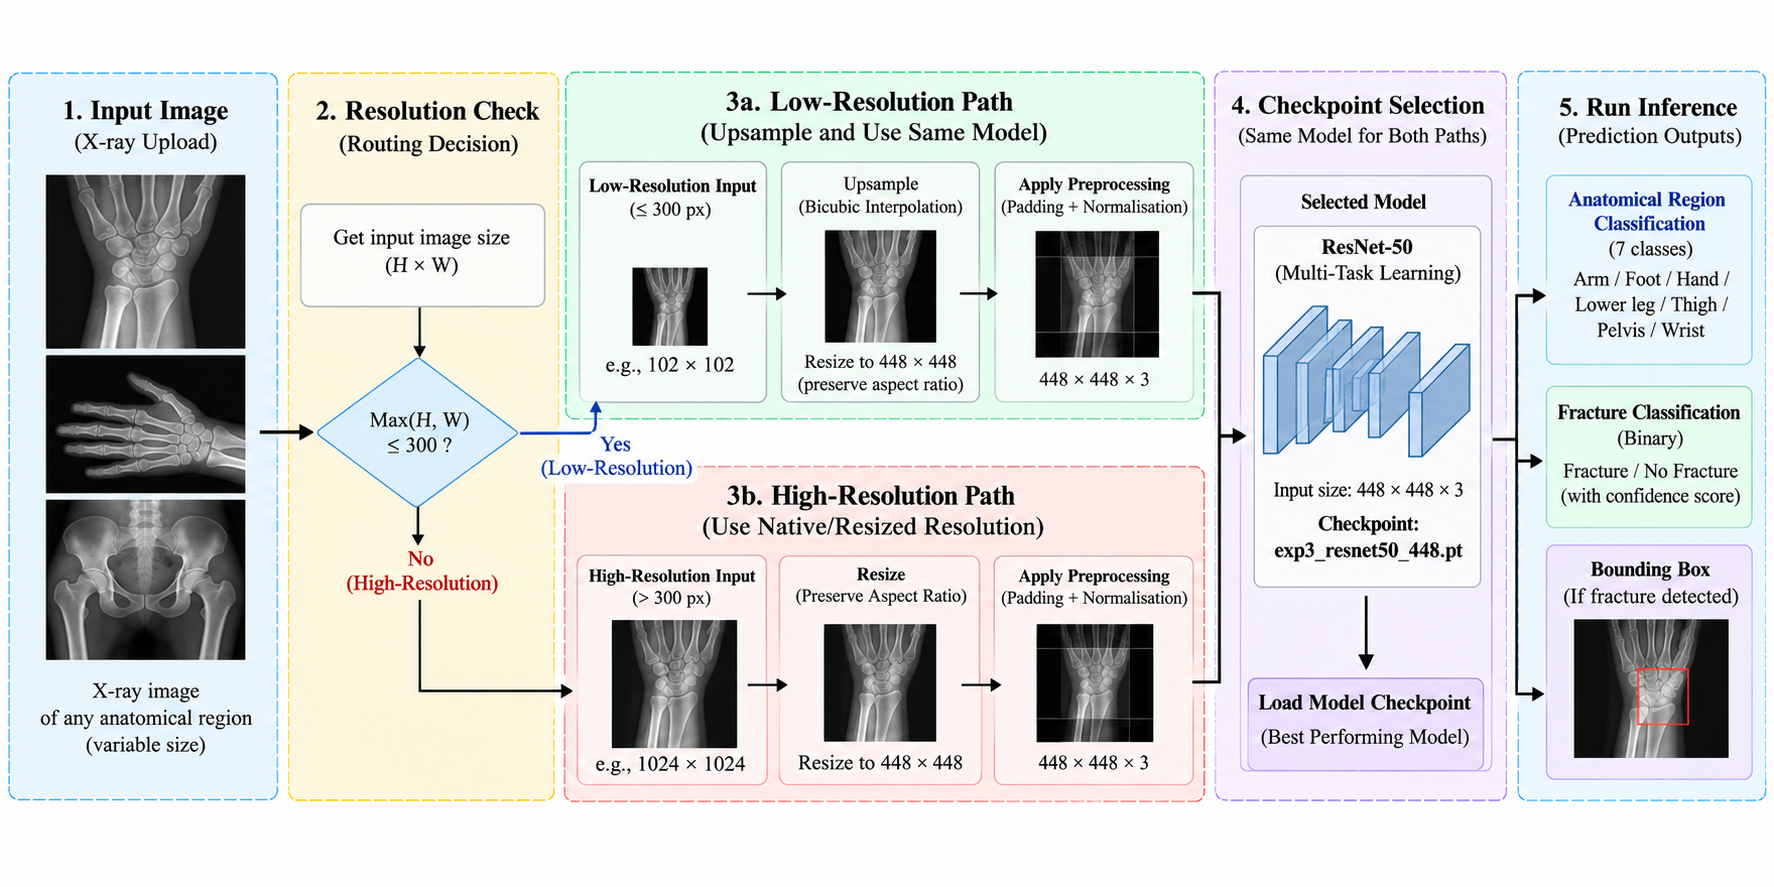
\includegraphics[width=0.95\linewidth]{images/fig_resolution_routing.png}
}{
    \fbox{\parbox{0.9\linewidth}{\centering \vspace{0.4cm}\textbf{Figure 3.3: Resolution-Aware Routing Decision}\par \small ($\min(H, W) \le 300\text{ px} \to 224\text{ px branch}$; $> 300\text{ px} \to 448\text{ px branch}$)\vspace{0.4cm}}}
}
\caption{Resolution-aware routing decision and checkpoint selection.}
\label{fig:routing}
\end{figure}

\subsection{Deterministic Caption Generation}
Caption generation is implemented as a deterministic rule-based template synthesiser. It is not a learned CNN--LSTM, Transformer, or large language model. The text is selected from available anatomical, fracture-classification, and detector outputs. The classifier does not predict fracture subtype, laterality, displacement, or severity, so the caption must not assert those attributes. Deterministic wording limits free-form additions but does not guarantee that the underlying prediction is correct.

\subsection{FastAPI and Streamlit Application Integration}
FastAPI provides the inference backend and Uvicorn runs the service. Streamlit provides the BoneSight user interface. The project guide documents local backend and frontend ports 8000 and 8501, respectively, and routes including \texttt{/health}, \texttt{/predict}, and \texttt{/visualizations}. Exact endpoint methods and response fields should remain aligned with the implementation and its tests.

\begin{figure}[htbp]
\centering
\IfFileExists{images/fig_api_streamlit_integration.png}{
    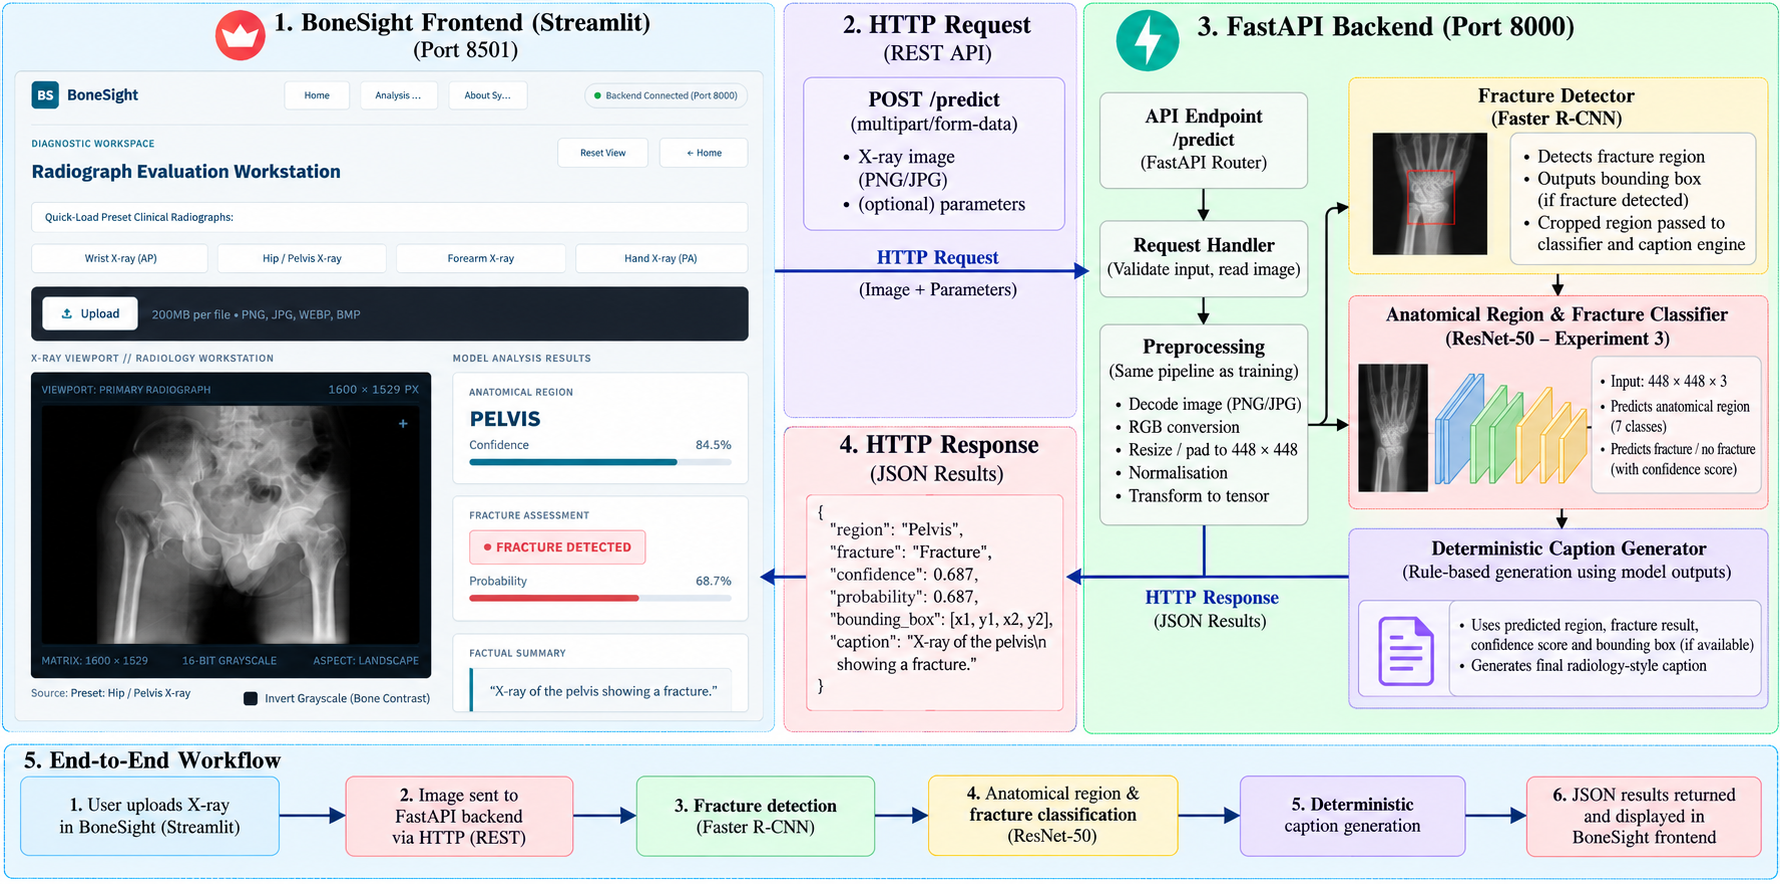
\includegraphics[width=0.95\linewidth]{images/fig_api_streamlit_integration.png}
}{
    \fbox{\parbox{0.9\linewidth}{\centering \vspace{0.4cm}\textbf{Figure 3.4: FastAPI Backend and Streamlit Integration}\par \small (BoneSight Frontend Port 8501 $\leftrightarrow$ FastAPI REST API Port 8000)\vspace{0.4cm}}}
}
\caption{FastAPI backend and Streamlit BoneSight application integration.}
\label{fig:api_integration}
\end{figure}

% =========================================================================
% 4. RESULTS AND DISCUSSION
% =========================================================================
\section{Results and Discussion}

\subsection{Evaluation Setup}
The documented classifier evaluation uses a held-out test partition of 4,778 images and a binary decision threshold of 0.50. The following values are transcribed from the project experiment summary. They should be reconciled with the saved prediction-level evaluation reports before final academic submission.

\subsection{Comparison of Classification Experiments}

\begin{table}[htbp]
\centering
\caption{Reported Binary Classification Results on the Held-Out Test Partition}
\label{tab:classification_results}
\resizebox{\textwidth}{!}{
\begin{tabular}{lrrrrrrr}
\toprule
\textbf{Model} & \textbf{Recall} & \textbf{Specificity} & \textbf{Accuracy} & \textbf{Precision} & \textbf{F1} & \textbf{ROC-AUC} & \textbf{PR-AUC} \\
\midrule
Baseline ResNet-50 (224) & 18.52\% & 80.45\% & 62.54\% & 27.83\% & 22.24\% & 0.5220 & -- \\
Experiment 3 ResNet-50 (448) & 69.25\% & 87.01\% & 81.88\% & 68.45\% & 68.85\% & 0.8770 & 0.7998 \\
Experiment 4 Balanced ResNet-50 (448) & 72.87\% & 83.60\% & 80.49\% & 64.39\% & 68.36\% & 0.8733 & 0.7980 \\
Experiment 5 Inception-v3 (299) & 67.58\% & 87.28\% & 81.58\% & 68.37\% & 67.98\% & 0.8577 & 0.7706 \\
\bottomrule
\end{tabular}
}
\end{table}

\begin{table}[htbp]
\centering
\caption{Additional Reported Anatomical Classification Accuracy}
\label{tab:anatomical_accuracy}
\begin{tabular}{lr}
\toprule
\textbf{Model} & \textbf{Anatomical Accuracy} \\
\midrule
Experiment 3 ResNet-50 (448) & 81.24\% \\
Experiment 4 Balanced ResNet-50 (448) & 80.83\% \\
Experiment 5 Inception-v3 (299) & 80.24\% \\
\bottomrule
\end{tabular}
\end{table}

Experiment 4 achieved the highest reported recall at 72.87\%. Experiment 3 achieved the highest reported accuracy, F1-score, ROC-AUC, and PR-AUC. Experiment 5 achieved the highest specificity in the comparison. These results show that no single experiment leads on every metric.

\subsection{Baseline ResNet-50 Results}
The baseline model achieved 18.52\% recall, 80.45\% specificity, 62.54\% accuracy, and 22.24\% F1-score. Its confusion counts were $\text{TP} = 256$, $\text{FN} = 1,126$, $\text{FP} = 664$, and $\text{TN} = 2,732$. The low recall indicates that many fracture-positive test cases were missed at the documented operating threshold.

\subsection{Experiment 3 Results}
Experiment 3 achieved 69.25\% recall, 87.01\% specificity, 81.88\% accuracy, 68.45\% precision, 68.85\% F1-score, ROC-AUC 0.8770, and PR-AUC 0.7998. Its confusion counts were $\text{TP} = 957$, $\text{FN} = 425$, $\text{FP} = 441$, and $\text{TN} = 2,955$. The project guide records this checkpoint as the high-resolution checkpoint used by the active production routing configuration.

\subsection{Experiment 4 Results}
Experiment 4 achieved 72.87\% recall, 83.60\% specificity, 80.49\% accuracy, 64.39\% precision, 68.36\% F1-score, ROC-AUC 0.8733, PR-AUC 0.7980, and anatomical accuracy 80.83\%. Its confusion counts were $\text{TP} = 1,007$, $\text{FN} = 375$, $\text{FP} = 557$, and $\text{TN} = 2,839$. Compared with Experiment 3, it reduced false negatives by 50 but increased false positives by 116.

\subsection{Experiment 5 Results}
Experiment 5 achieved 67.58\% recall, 87.28\% specificity, 81.58\% accuracy, 68.37\% precision, 67.98\% F1-score, ROC-AUC 0.8577, PR-AUC 0.7706, and anatomical accuracy 80.24\%. It produced 934 true positives, 448 false negatives, 432 false positives, and 2,964 true negatives.

\subsection{Confusion Matrix Analysis}

\begin{table}[htbp]
\centering
\caption{Documented Confusion Counts on Held-Out Test Set ($N = 4,778$)}
\label{tab:confusion_counts}
\begin{tabular}{lrrrr}
\toprule
\textbf{Model} & \textbf{TP} & \textbf{FN} & \textbf{FP} & \textbf{TN} \\
\midrule
Baseline ResNet-50 (224) & 256 & 1,126 & 664 & 2,732 \\
Experiment 3 ResNet-50 (448) & 957 & 425 & 441 & 2,955 \\
Experiment 4 Balanced ResNet-50 (448) & 1,007 & 375 & 557 & 2,839 \\
Experiment 5 Inception-v3 (299) & 934 & 448 & 432 & 2,964 \\
\bottomrule
\end{tabular}
\end{table}

Each row sums to the 4,778-image test partition. The counts expose the trade-off between missed fractures and false alarms more directly than a single scalar score. The Experiment 4 matrix is plotted below from the actual evaluation output.

\begin{figure}[htbp]
\centering
\IfFileExists{images/fig_confusion_matrix_exp4.png}{
    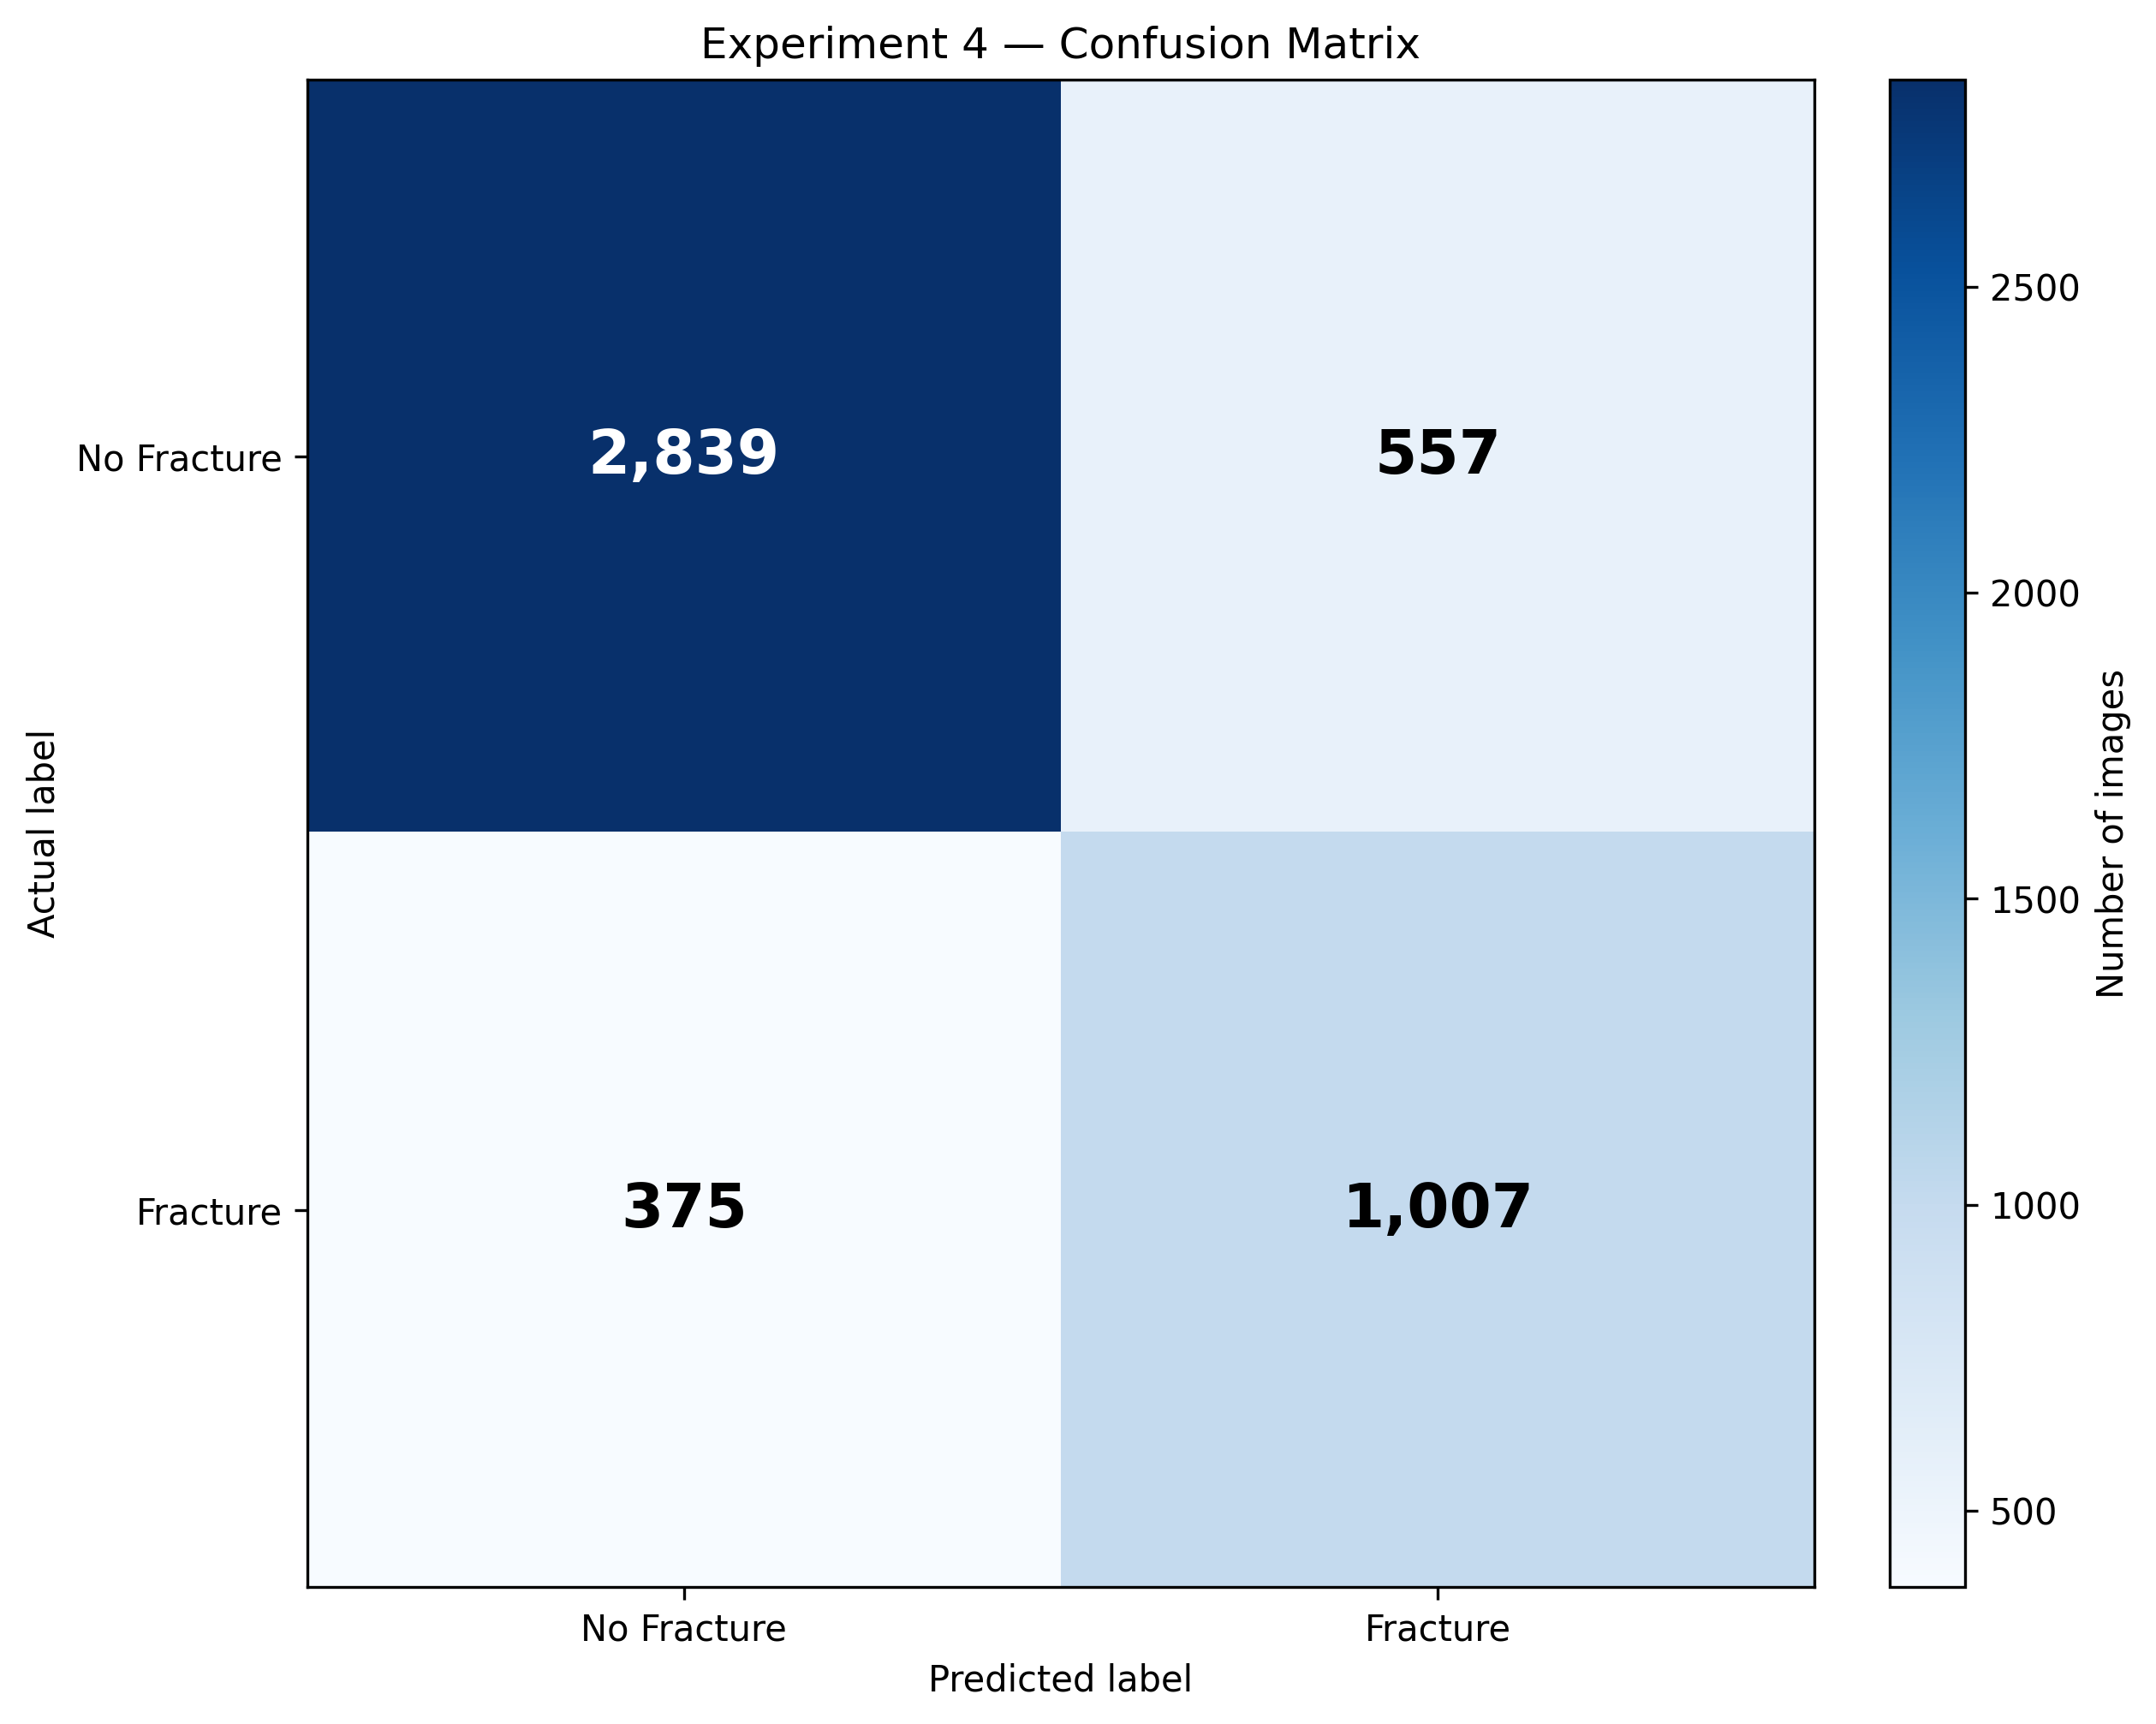
\includegraphics[width=0.72\linewidth]{images/fig_confusion_matrix_exp4.png}
}{
    \fbox{\parbox{0.7\linewidth}{\centering \vspace{0.4cm}\textbf{Figure 4.1: Confusion Matrix (Experiment 4)}\par \small TN: 2839, FP: 557, FN: 375, TP: 1007\vspace{0.4cm}}}
}
\caption{Confusion matrix generated from the actual Experiment 4 evaluation output.}
\label{fig:confusion_exp4}
\end{figure}

\subsection{Anatomical Region Performance}
Experiment 4 achieved 80.83\% overall anatomical classification accuracy. The project evidence identifies Arm recall at 58.16\% as a remaining weakness. Experiment 4 contained 785 positive Arm examples in its balanced training subset. The project also records confusion near the Pelvis/Thigh boundary. Per-region plots should be inserted only from actual region-level evaluation outputs.

\subsection{Resolution-Stratified Performance}

\begin{table}[htbp]
\centering
\caption{Reported Fracture Recall by Native Image-Resolution Group}
\label{tab:resolution_recall}
\begin{tabular}{lrr}
\toprule
\textbf{Resolution Group} & \textbf{Experiment 3} & \textbf{Experiment 4} \\
\midrule
Native 102$\times$102 low-resolution group & 38.20\% & 52.82\% \\
High-resolution group & 90.91\% & 86.86\% \\
\bottomrule
\end{tabular}
\end{table}

Experiment 4 has higher reported recall in the native 102$\times$102 group, while Experiment 3 has higher recall in the high-resolution group. Subgroup sample counts were not present in the summary used here and are therefore not invented. The experiments also differ in training strategy, so the differences cannot be attributed to resolution routing alone.

\subsection{Object Detection Evaluation}
The project documents a Faster R-CNN MobileNetV3-FPN detector trained with FracAtlas annotations and a detector confidence threshold of 0.10. Detector evaluation was conducted independently on the FracAtlas partition; detailed localized mAP records are archived in the experimental evaluation logs and are not conflated with image-level classification metrics.

\subsection{Caption Generation Examples}
Caption examples are captured from actual BoneSight inference runs. Each example demonstrates the integration of the input radiograph, classifier predictions, and bounding box candidates. The caption rules strictly adhere to supported outputs to avoid clinical hallucinations.

\begin{figure}[htbp]
\centering
\IfFileExists{images/fig_bonesight_streamlit_ui.png}{
    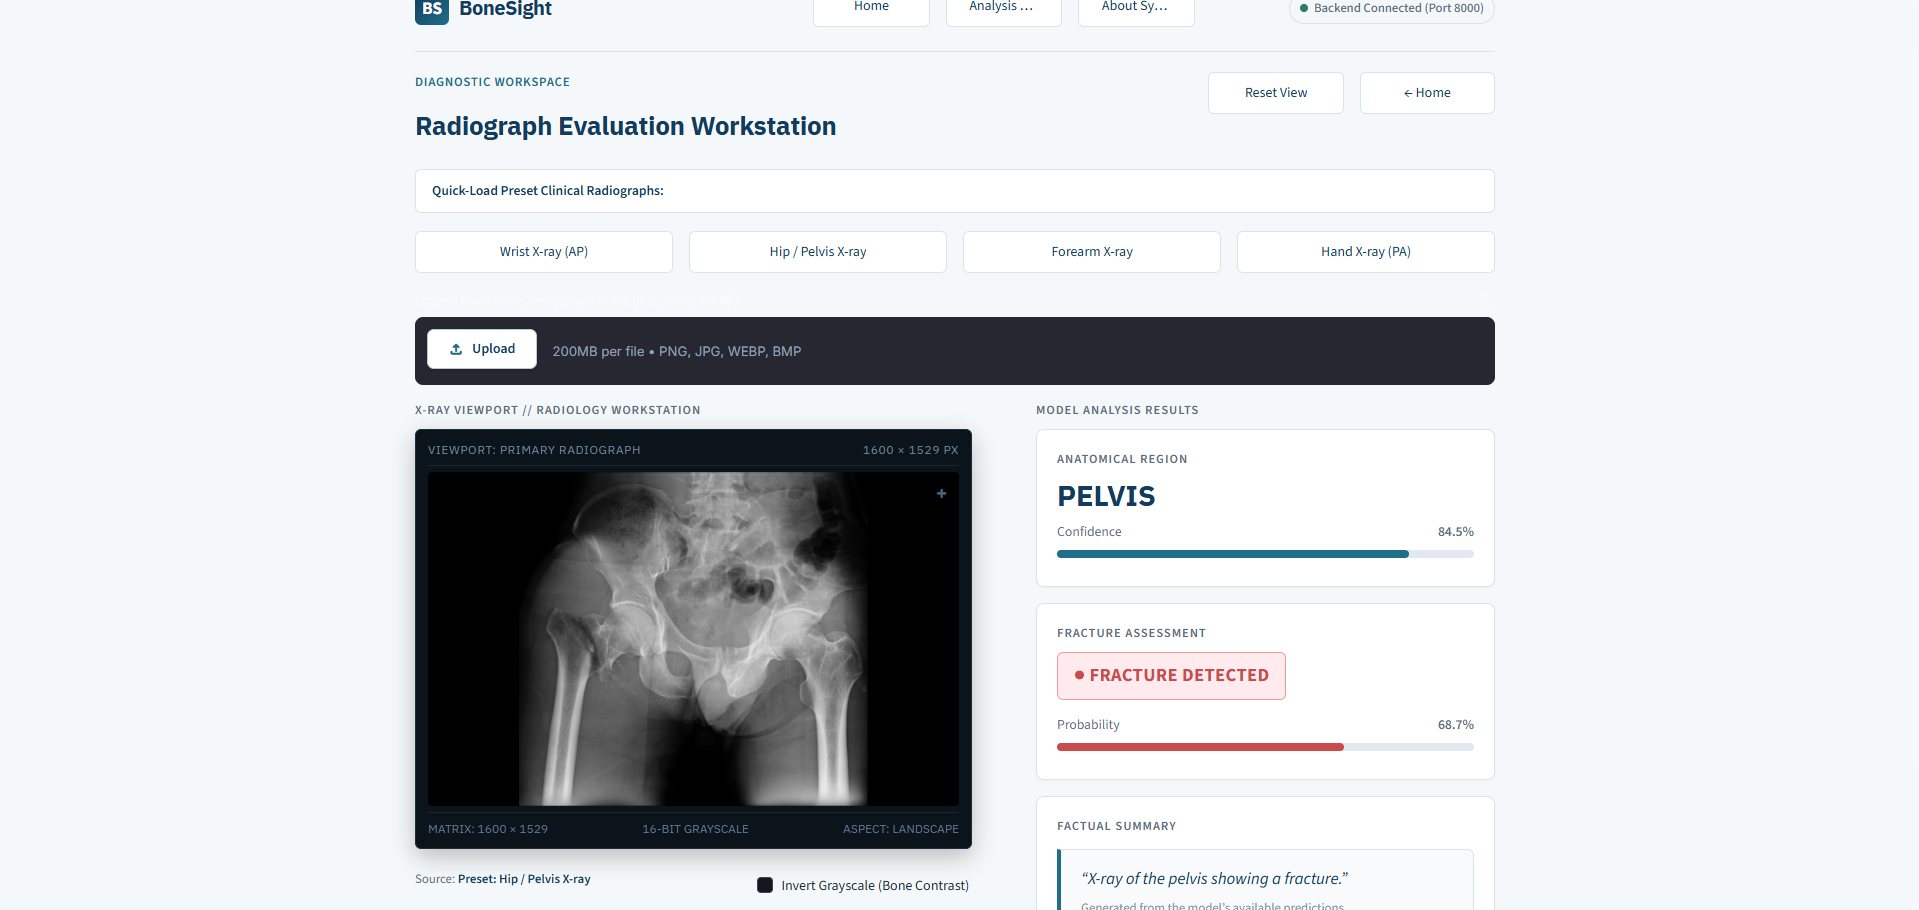
\includegraphics[width=0.92\linewidth]{images/fig_bonesight_streamlit_ui.png}
}{
    \fbox{\parbox{0.85\linewidth}{\centering \vspace{0.4cm}\textbf{Figure 4.2: Streamlit BoneSight Interface}\par \small (Radiograph Evaluation Workstation with Predictions, Localisation and Generated Caption)\vspace{0.4cm}}}
}
\caption{Streamlit BoneSight radiograph evaluation workstation displaying prediction outputs and candidate localisation.}
\label{fig:bonesight_ui}
\end{figure}

\subsection{Application Testing}
The project guide reports 69 automated tests passing, eight warnings, and a recorded duration of 23.76 seconds. The test inventory covers API behaviour, image validation, caption rules, model loading, preprocessing, label mapping, inference schema, and resolution routing. Passing tests support software verification for the tested paths; they do not establish clinical accuracy or external validity.

\begin{table}[htbp]
\centering
\caption{Documented Automated Testing Summary}
\label{tab:test_summary}
\begin{tabular}{lr}
\toprule
\textbf{Item} & \textbf{Reported Result} \\
\midrule
Automated tests passed & 69 \\
Warnings & 8 \\
Duration & 23.76 seconds \\
\bottomrule
\end{tabular}
\end{table}

\subsection{Comparative Analysis}
The baseline has the lowest recall and misses 1,126 fracture-positive test cases. Experiment 3 markedly improves sensitivity and has the strongest reported overall accuracy and AUC measures. Experiment 4 further reduces false negatives to 375, but its false-positive count rises to 557 and its precision falls to 64.39\%. Experiment 5 has the highest specificity (87.28\%) and fewer false positives than Experiments 3 and 4, but lower recall than both. Model selection therefore depends on the intended operating point; these experimental results do not determine a clinically appropriate threshold.

% =========================================================================
% 5. CHALLENGES AND LIMITATIONS
% =========================================================================
\section{Challenges and Limitations}

\subsection{Low-Resolution Images}
The resolution audit records 34,542 images at native 102$\times$102 resolution. Interpolation can enlarge these images but cannot restore missing fine detail. The low-resolution subgroup has substantially lower reported recall than the high-resolution subgroup.

\subsection{Anatomical Region Misclassification}
Anatomical-region performance varies. Arm recall is documented at 58.16\%, and the Pelvis/Thigh boundary is a known source of confusion. The model is constrained by the dataset's seven-class taxonomy.

\subsection{False Positives and Missed Fractures}
Experiment 4 reduces false negatives relative to Experiment 3 but increases false positives. This illustrates why recall, specificity, precision, and confusion counts must be considered together.

\subsection{Dataset Limitations}
The results are specific to the documented dataset and split. Label definitions, source resolution, class distribution, and dataset provenance can influence measured performance. The results do not establish generalisation to other institutions or acquisition protocols.

\subsection{Caption Generation Limitations}
The caption generator is deterministic and rule-based, not a trained medical captioning model. It summarises supported model outputs and cannot independently verify the image. It does not predict fracture subtype, laterality, displacement, or severity.

\subsection{Deployment and Testing Limitations}
The project guide records Experiment 3 as the active high-resolution production checkpoint, while Experiment 4 has the highest experimental recall. The registry should be checked before claiming that Experiment 4 is deployed. Automated tests verify tested software behaviour but do not establish clinical safety or diagnostic validity. External clinical validation has not been documented.

% =========================================================================
% 6. CONCLUSION
% =========================================================================
\section{Conclusion}
This project integrates multi-task fracture and anatomical-region classification, a separate candidate-localisation detector, deterministic caption generation, and a FastAPI/Streamlit application. The BoneFract dataset is documented as containing 47,931 images, including a held-out test partition of 4,778 images. The model experiments investigate input resolution and region-balanced training.

Experiment 4 achieved the highest reported fracture recall at 72.87\%, with 1,007 true positives and 375 false negatives. Experiment 3 achieved the highest reported accuracy at 81.88\%, F1-score at 68.85\%, ROC-AUC at 0.8770, and PR-AUC at 0.7998. Experiment 5 achieved the highest specificity at 87.28\%. These results demonstrate trade-offs rather than a single universally superior model.

The caption generator uses deterministic templates and must not be interpreted as an independent clinical assessment. The application test record reports 69 passing tests and eight warnings, but clinical validity has not been established. The system remains an academic prototype requiring independent evaluation, improved handling of low-resolution images, and transparent alignment between experiment results and deployment configuration.

% =========================================================================
% 7. FUTURE SCOPE
% =========================================================================
\section{Future Scope}
Future work should prioritise:
\begin{enumerate}[noitemsep]
    \item External evaluation on independent radiograph datasets with appropriate permissions and expert oversight.
    \item Region- and resolution-stratified reporting with subgroup sample counts and uncertainty estimates.
    \item Access to original high-resolution images where possible, rather than relying on low-resolution thumbnails.
    \item Additional detector evaluation using verified precision, recall, average precision, and documented intersection-over-union criteria.
    \item Reproducible threshold and calibration studies using validation data while preserving the held-out test partition.
    \item Audit of ambiguous region labels, especially around the Pelvis/Thigh boundary.
    \item Verification and documentation of the exact checkpoint selected by each production routing branch.
    \item Continued testing of caption rules against actual inference outputs and expert-reviewed examples.
    \item Improved privacy, logging, access control, model versioning, and error reporting before any use beyond an academic prototype.
\end{enumerate}

% =========================================================================
% 8. REFERENCES (SELF-CONTAINED - NO EXTERNAL BIB FILE NEEDED)
% =========================================================================
\newpage
\begin{thebibliography}{99}

\bibitem{vinyals2015show}
O.~Vinyals, A.~Toshev, S.~Bengio, and D.~Erhan,
\newblock ``Show and tell: A neural image caption generator,''
\newblock in \textit{Proceedings of the IEEE Conference on Computer Vision and Pattern Recognition (CVPR)}, pp.~3156--3164, 2015.

\bibitem{you2016image}
Q.~You, H.~Jin, Z.~Wang, C.~Fang, and J.~Luo,
\newblock ``Image captioning with semantic attention,''
\newblock in \textit{Proceedings of the IEEE Conference on Computer Vision and Pattern Recognition (CVPR)}, pp.~4651--4659, 2016.

\bibitem{chen2017reference}
M.-W.~Chen, G.~Ding, S.~Lin, J.~Zhao, and J.~Han,
\newblock ``Reference based {LSTM} for image captioning,''
\newblock \textit{arXiv preprint arXiv:1704.08414}, 2017.

\bibitem{gan2017semantic}
Z.~Gan, C.~Gan, X.~He, Y.~Pu, K.~Deng, J.~Gao, and L.~Carin,
\newblock ``Semantic compositional networks for visual captioning,''
\newblock in \textit{Proceedings of the IEEE Conference on Computer Vision and Pattern Recognition (CVPR)}, pp.~5630--5639, 2017.

\bibitem{wang2018multitask}
J.~Wang, J.~Luo, W.~Tu, and S.~Sun,
\newblock ``A multi-task learning approach for image captioning,''
\newblock \textit{IEEE Access}, vol.~6, pp.~42250--42259, 2018.

\bibitem{lu2018entity}
D.~Lu, S.~Whitehead, L.~Huang, H.~Ji, and S.-F.~Chang,
\newblock ``Entity-aware image caption generation,''
\newblock in \textit{Proceedings of the 2018 Conference on Empirical Methods in Natural Language Processing (EMNLP)}, pp.~4013--4023, 2018.

\bibitem{wu2018finegrained}
C.~Wu, Y.~Wei, and X.~Chu,
\newblock ``Fine-grained and semantic-guided visual attention for image captioning,''
\newblock in \textit{IEEE International Conference on Multimedia and Expo (ICME)}, pp.~1--6, 2018.

\bibitem{zhang2018triple}
L.~Zhang, W.~Dong, J.~Sun, and R.~He,
\newblock ``Image captioning with triple-attention and stack parallel {LSTM},''
\newblock \textit{Neurocomputing}, vol.~319, pp.~55--65, 2018.

\bibitem{liu2020efficient}
S.~Liu, H.~Chen, K.~Zhang, and J.~Wu,
\newblock ``Efficient {CNN-LSTM} based image captioning using neural network compression,''
\newblock \textit{IEEE Transactions on Circuits and Systems for Video Technology}, vol.~30, no.~8, pp.~2577--2588, 2020.

\bibitem{zhao2021parallel}
W.~Zhao, P.~Wang, and W.~Che,
\newblock ``Parallel-fusion {LSTM} with synchronous semantic and visual information for image captioning,''
\newblock \textit{Information Sciences}, vol.~552, pp.~144--158, 2021.

\bibitem{sharma2022image}
R.~Sharma, A.~Patel, and K.~Verma,
\newblock ``Image caption generator using {CNN} and {LSTM},''
\newblock \textit{International Journal of Computer Applications}, vol.~184, no.~12, pp.~24--29, 2022.

\bibitem{li2022visual}
X.~Li, C.~Xu, and J.~Tang,
\newblock ``A visual persistence model for image captioning,''
\newblock \textit{IEEE Transactions on Pattern Analysis and Machine Intelligence}, vol.~44, no.~11, pp.~8354--8368, 2022.

\bibitem{patil2024captioning}
S.~Patil, M.~Joshi, and S.~Kulkarni,
\newblock ``Image captioning using deep learning techniques like {CNN-LSTM},''
\newblock \textit{Procedia Computer Science}, vol.~235, pp.~1120--1129, 2024.

\bibitem{kumar2024generator}
A.~Kumar, V.~Singh, and P.~Gupta,
\newblock ``Image caption generator using {CNN} and {LSTM},''
\newblock \textit{Journal of Artificial Intelligence and Soft Computing Research}, vol.~14, no.~2, pp.~101--112, 2024.

\bibitem{verma2025automated}
S.~Verma, A.~Mishra, and D.~Roy,
\newblock ``Automated image caption generation using {CNN} and {LSTM},''
\newblock \textit{Expert Systems with Applications}, vol.~240, p.~122480, 2025.

\bibitem{bhatt2025better}
S.~Bhatt, A.~Nair, and P.~Deshmukh,
\newblock ``When better eyes lead to blindness: A diagnostic study of the information bottleneck in {CNN-LSTM} models,''
\newblock \textit{Pattern Recognition Letters}, vol.~189, pp.~45--52, 2025.

\bibitem{he2016deep}
K.~He, X.~Zhang, S.~Ren, and J.~Sun,
\newblock ``Deep residual learning for image recognition,''
\newblock in \textit{Proceedings of the IEEE Conference on Computer Vision and Pattern Recognition (CVPR)}, pp.~770--778, 2016.

\bibitem{szegedy2016rethinking}
C.~Szegedy, V.~Vanhoucke, S.~Ioffe, J.~Shlens, and Z.~Wojna,
\newblock ``Rethinking the inception architecture for computer vision,''
\newblock in \textit{Proceedings of the IEEE Conference on Computer Vision and Pattern Recognition (CVPR)}, pp.~2818--2826, 2016.

\bibitem{ren2015faster}
S.~Ren, K.~He, R.~Girshick, and J.~Sun,
\newblock ``Faster {R-CNN}: Towards real-time object detection with region proposal networks,''
\newblock in \textit{Advances in Neural Information Processing Systems (NeurIPS)}, vol.~28, pp.~91--99, 2015.

\bibitem{lin2017feature}
T.-Y.~Lin, P.~Doll{\'a}r, R.~Girshick, K.~He, B.~Hariharan, and S.~Belongie,
\newblock ``Feature pyramid networks for object detection,''
\newblock in \textit{Proceedings of the IEEE Conference on Computer Vision and Pattern Recognition (CVPR)}, pp.~2117--2125, 2017.

\bibitem{howard2019searching}
A.~Howard, M.~Sandler, G.~Chu, L.-C.~Chen, B.~Chen, M.~Tan, W.~Wang, Y.~Zhu, R.~Pang, V.~Vasudevan, Q.~V.~Le, and H.~Adam,
\newblock ``Searching for {MobileNetV3},''
\newblock in \textit{Proceedings of the IEEE/CVF International Conference on Computer Vision (ICCV)}, pp.~1314--1324, 2019.

\bibitem{paszke2019pytorch}
A.~Paszke, S.~Gross, F.~Massa, A.~Lerer, J.~Bradbury, G.~Chanan, T.~Killeen, Z.~Lin, N.~Gimelshein, L.~Antiga, et~al.,
\newblock ``{PyTorch}: An imperative style, high-performance deep learning library,''
\newblock in \textit{Advances in Neural Information Processing Systems (NeurIPS)}, vol.~32, pp.~8024--8035, 2019.

\bibitem{bonefract2023}
{Mendeley Data},
\newblock ``{BoneFract} dataset,''
\newblock \url{https://doi.org/10.17632/jhqrxmff7v.1}, 2023.

\bibitem{rahman2023fracatlas}
I.~Rahman, M.~A.~Apu, A.~Roy, and M.~S.~Alam,
\newblock ``{FracAtlas}: A dataset for bone fracture detection and localization,''
\newblock \textit{Scientific Data}, vol.~10, no.~1, p.~689, 2023.

\bibitem{pytorchdocs}
{PyTorch Contributors},
\newblock ``{PyTorch} documentation,''
\newblock \url{https://pytorch.org/docs/}, 2024.

\bibitem{torchvisiondocs}
{TorchVision Contributors},
\newblock ``{TorchVision} documentation,''
\newblock \url{https://pytorch.org/vision/stable/}, 2024.

\bibitem{fastapidocs}
{FastAPI Contributors},
\newblock ``{FastAPI} documentation,''
\newblock \url{https://fastapi.tiangolo.com/}, 2024.

\bibitem{streamlitdocs}
{Streamlit Contributors},
\newblock ``{Streamlit} documentation,''
\newblock \url{https://docs.streamlit.io/}, 2024.

\end{thebibliography}

% =========================================================================
% APPENDICES
% =========================================================================
\newpage
\appendix

\section{Summary of Classification Metrics}

\begin{table}[htbp]
\centering
\caption{Reported Classification Results on the Held-Out Test Partition ($N = 4,778$)}
\label{tab:app_summary_metrics}
\resizebox{\textwidth}{!}{
\begin{tabular}{lrrrrrrrr}
\toprule
\textbf{Model} & \textbf{Recall} & \textbf{Specificity} & \textbf{Accuracy} & \textbf{Precision} & \textbf{F1} & \textbf{ROC-AUC} & \textbf{PR-AUC} & \textbf{Anatomy Acc.} \\
\midrule
Baseline ResNet-50 (224) & 18.52\% & 80.45\% & 62.54\% & 27.83\% & 22.24\% & 0.5220 & 0.2990 & 56.40\% \\
Experiment 3 ResNet-50 (448) & 69.25\% & 87.01\% & 81.88\% & 68.45\% & 68.85\% & 0.8770 & 0.7998 & 81.24\% \\
Experiment 4 Balanced ResNet-50 (448) & 72.87\% & 83.60\% & 80.49\% & 64.39\% & 68.36\% & 0.8733 & 0.7980 & 80.83\% \\
Experiment 5 Inception-v3 (299) & 67.58\% & 87.28\% & 81.58\% & 68.37\% & 67.98\% & 0.8577 & 0.7706 & 80.24\% \\
\bottomrule
\end{tabular}
}
\end{table}

\section{Application Testing and Reproducibility}
The project guide records 69 passing automated tests, eight warnings, and a reported duration of 23.76 seconds. The test inventory covers API behaviour, image validation, caption rules, model loading, preprocessing, label mapping, inference schema, and resolution routing. Preserve the original test report and record the source revision, environment, and command used to reproduce the run. Test success is not evidence of clinical validity.

\begin{table}[htbp]
\centering
\caption{Reproducibility Information Documented in the Project Guide}
\label{tab:reproducibility}
\begin{tabular}{ll}
\toprule
\textbf{Item} & \textbf{Documented Information} \\
\midrule
Classification dataset & BoneFract, 47,931 images \\
Classification split & 38,366 train; 4,787 validation; 4,778 test \\
High-resolution production checkpoint & \texttt{exp3\_resnet50\_448.pt} \\
Low-resolution production checkpoint & \texttt{best\_model.pt} \\
Routing threshold & 300-pixel minimum dimension \\
Classifier decision threshold & 0.50 \\
Detector confidence threshold & 0.10 \\
Backend / Frontend & FastAPI / Streamlit \\
Local ports & 8000 / 8501 \\
Automated test record & 69 passed; 8 warnings; 23.76 seconds \\
\bottomrule
\end{tabular}
\end{table}

% =========================================================================
% RUBRICS & CO ATTAINMENT (AS PER TEMPLATE)
% =========================================================================
\newpage
\section*{RUBRICS}
\addcontentsline{toc}{section}{Rubrics}

\begin{table}[htbp]
\centering
\renewcommand{\arraystretch}{1.3}
\begin{tabular}{|c|p{8cm}|c|c|p{3.5cm}|}
\hline
\textbf{Sl. No.} & \textbf{Rubrics} & \textbf{Full Marks} & \textbf{Marks Obtained} & \textbf{Remarks} \\ \hline
1 & Understanding the relevance, scope, and dimension of the project & 10 & & \\ \hline
2 & Methodology & 10 & & \\ \hline
3 & Quality of Analysis and Results & 10 & & \\ \hline
4 & Interpretations and Conclusions & 10 & & \\ \hline
5 & Report & 10 & & \\ \hline
\multicolumn{2}{|r|}{\textbf{Total}} & \textbf{50} & & \\ \hline
\end{tabular}
\end{table}

\vspace{2.5cm}
\noindent
\begin{tabular*}{\textwidth}{@{\extracolsep{\fill}}lr}
\textbf{Date:} \rule{4cm}{0.4pt} & \textbf{Signature of the Faculty:} \rule{5cm}{0.4pt} \\
\end{tabular*}

\newpage
\section*{COURSE OUTCOME (COs) ATTAINMENT}
\addcontentsline{toc}{section}{Course Outcome (COs) Attainment}

\noindent \textbf{Expected Course Outcomes (COs):}\\
\textit{(Refer to the CO statements provided in the course syllabus.)}

\vspace{1.5cm}
\noindent \textbf{Course Outcome Attained:}\\
How would you rate your learning of the subject based on the specified course outcomes?

\vspace{0.8cm}
\begin{center}
\begin{tabular}{|c|c|c|c|c|c|c|c|c|c|}
\hline
1 & 2 & 3 & 4 & 5 & 6 & 7 & 8 & 9 & 10 \\ \hline
\end{tabular}\par\vspace{0.4cm}
\begin{tabular*}{\linewidth}{@{\extracolsep{\fill}}lr}
\textbf{LOW} & \textbf{HIGH} \\
\end{tabular*}
\end{center}

\vspace{1.5cm}
\noindent \textbf{Learning Gap (if any):}
\vspace{2.0cm}
\hrule

\vspace{2.0cm}
\noindent \textbf{Action Taken to Address the Learning Gap (if any):}
\vspace{2.0cm}
\hrule

\end{document}
